\section{Application Layer}

\subsection{Principles of network applications}


\key{TCP 4-tuple}
\begin{itemize}
  \item Source $\langle$IP, Port$\rangle$
  \item Dest $\langle$IP, Port$\rangle$
\end{itemize}

\key{What transport service does an app need?}
\begin{figure}[H]
  \centering
  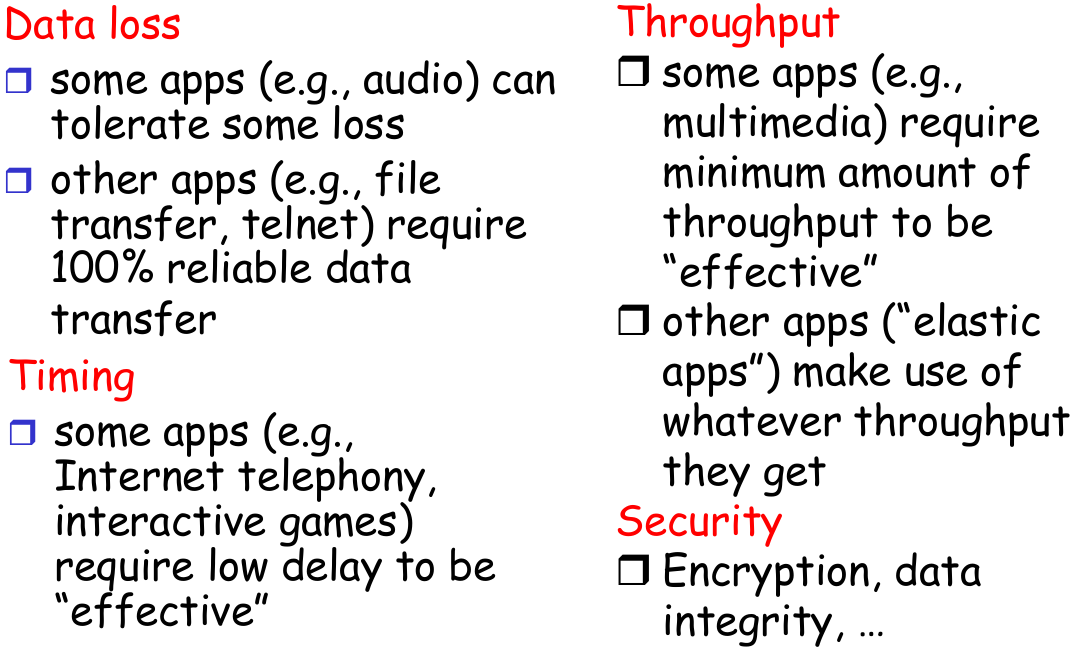
\includegraphics[width=0.5\textwidth]{transport}
\end{figure}

\subsection{Web and HTTP}

\key{HTTP connections}
\begin{figure}[H]
  \centering
  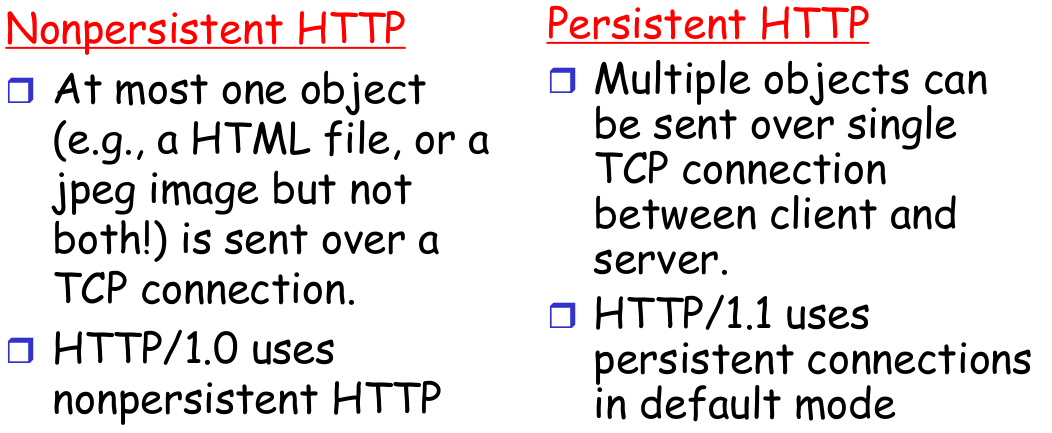
\includegraphics[width=0.5\textwidth]{http_conn}
\end{figure}

\key{Non-Persistent HTTP Response time modeling}
\begin{figure}[H]
  \centering
  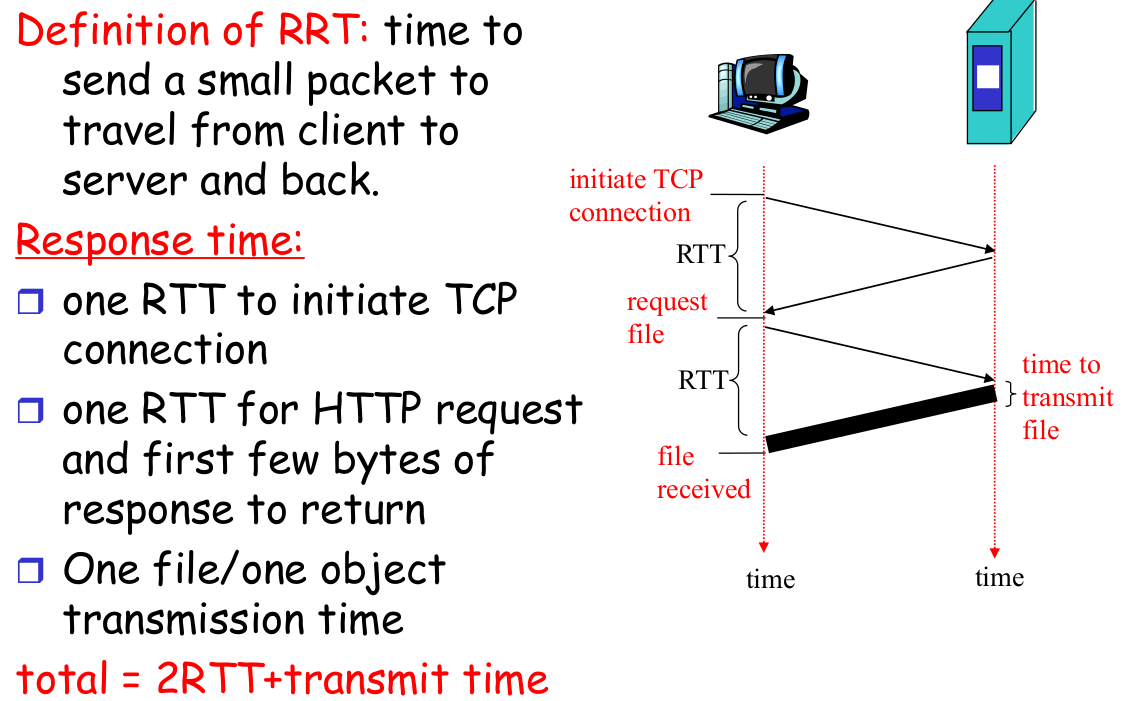
\includegraphics[width=0.5\textwidth]{http}
\end{figure}

\key{Web caches (proxy server) and CDN}
\begin{figure}[H]
  \centering
  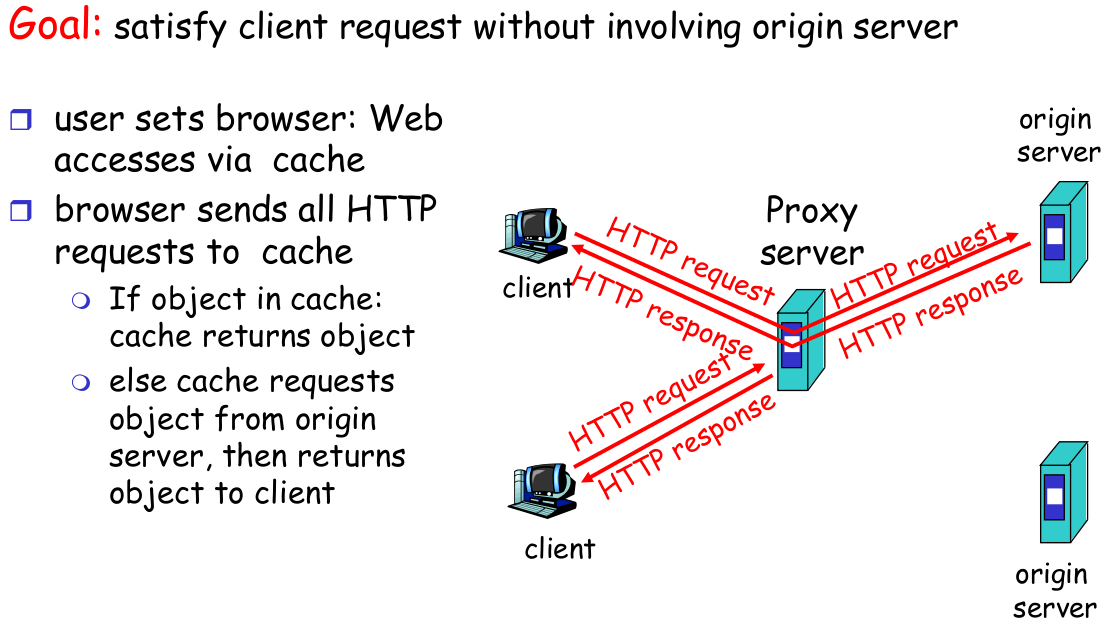
\includegraphics[width=0.48\textwidth]{proxy}
  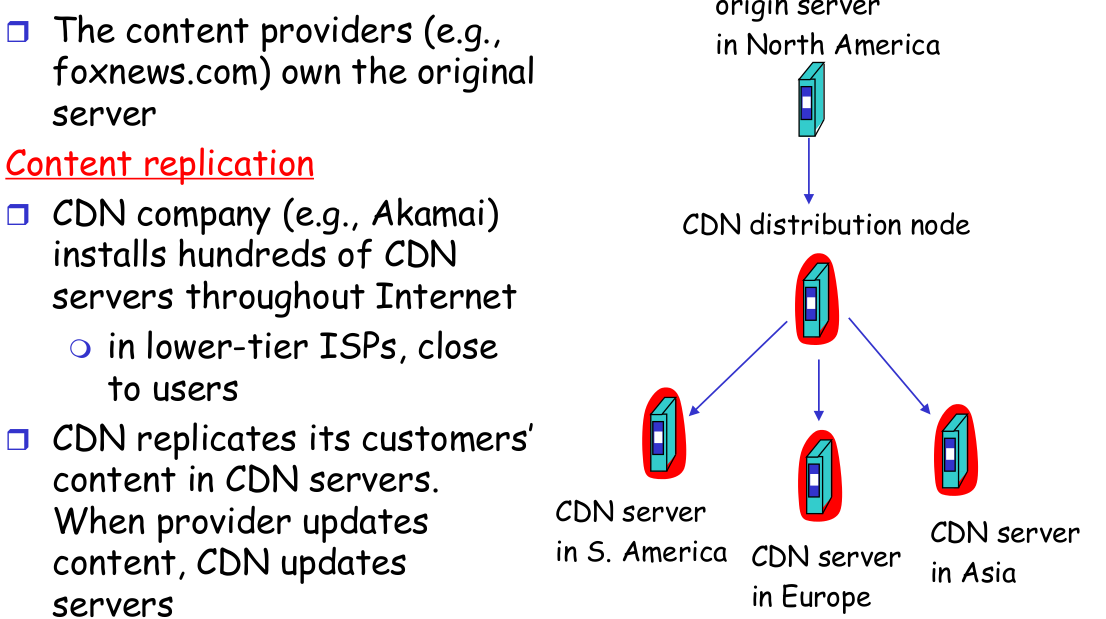
\includegraphics[width=0.48\textwidth]{cdn}
\end{figure}

\subsection{FTP}

\key{FTP: separate control, data connections}
\begin{figure}[H]
  \centering
  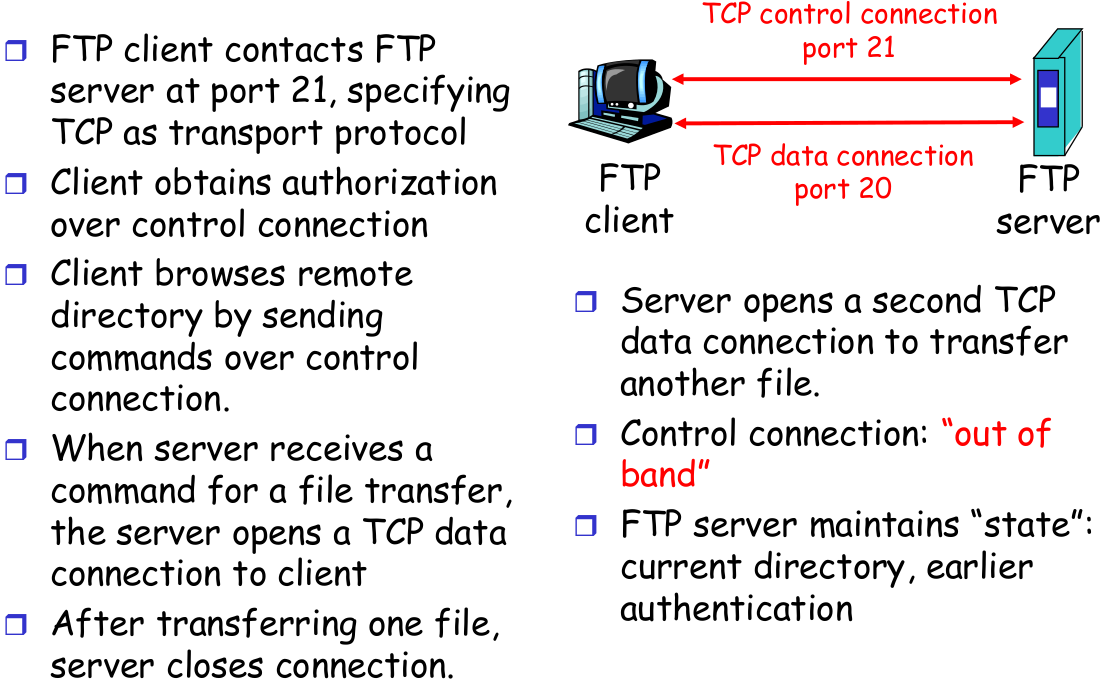
\includegraphics[width=0.48\textwidth]{ftp}
\end{figure}

\subsection{DNS}

\key{DNS: Domain Name System}
\begin{figure}[H]
  \centering
  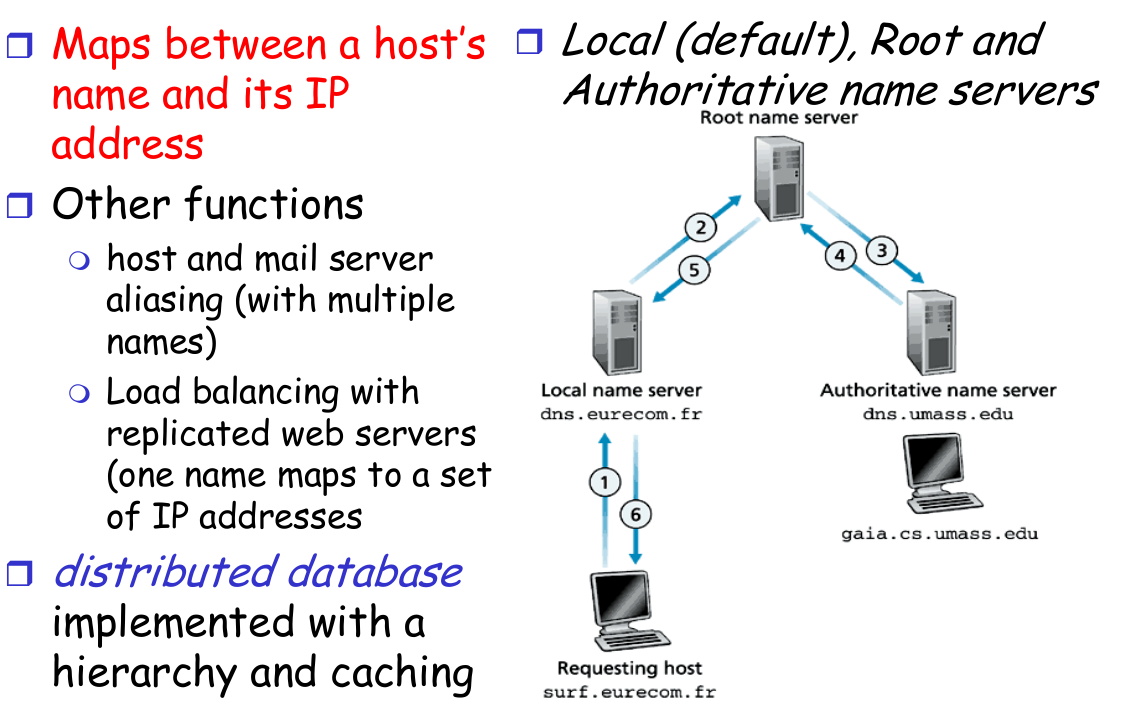
\includegraphics[width=0.48\textwidth]{dns}
\end{figure}


\subsection{P2P applications}

\key{File distribution time: server-client vs. P2P}
\begin{figure}[H]
  \centering
  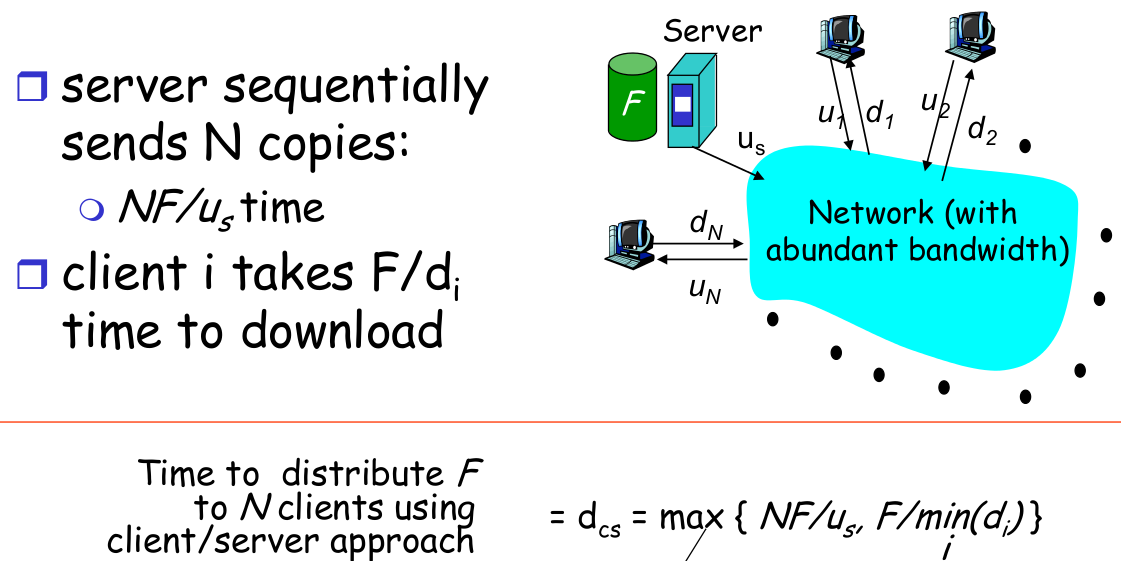
\includegraphics[width=0.48\textwidth]{file-cs}
  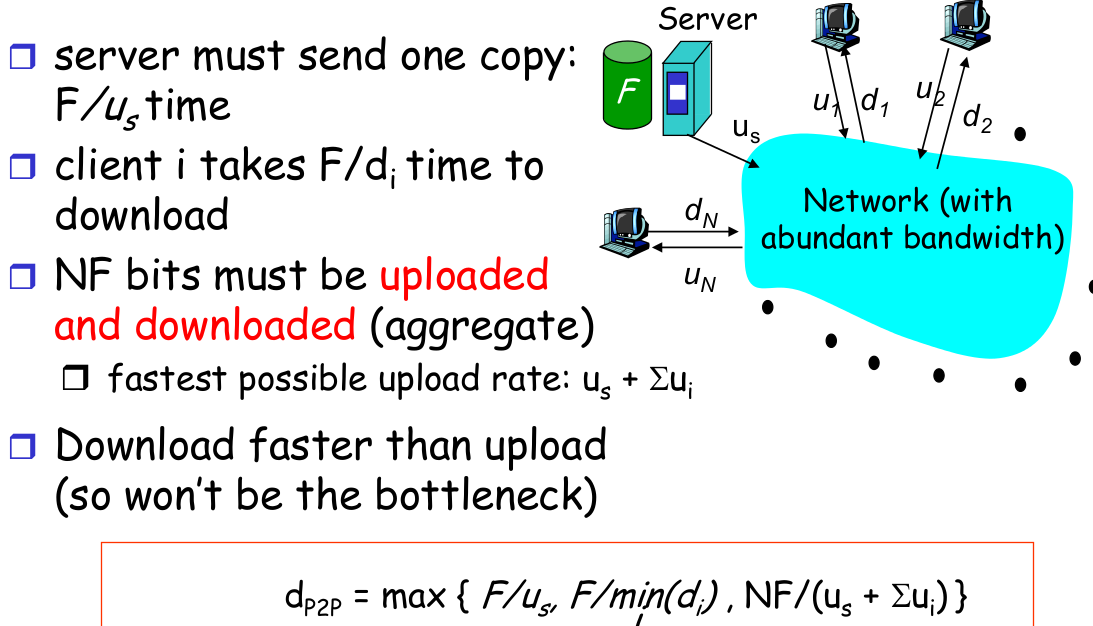
\includegraphics[width=0.48\textwidth]{file-p2p}
\end{figure}

\key{Optimistically Unchoke}
\begin{itemize}
  \item Alice sends chunks to four neighbors currently
    sending her chunks at the highest rate
  \item Re-evaluate top 4 every 10 secs
  \item  Every 30 secs: randomly select another peer, starts sending chunks
  \item Newly chosen peer may join top 4
\end{itemize}


